\documentclass[dvipdfmx,autodetect-engine,titlepage]{jsarticle}
\usepackage[dvipdfm]{graphicx}
\usepackage{ascmac}
\usepackage{fancybox}
\usepackage{listings}
\usepackage{plistings}
\usepackage{itembkbx}
\usepackage{amsmath}
\usepackage{url}
\usepackage{graphics}
\usepackage{listings}
\usepackage{here}

\lstset{%
  language={C},
  basicstyle={\small},%
  identifierstyle={\small},%
  commentstyle={\small\itshape\color[rgb]{0,0.5,0}},%
  keywordstyle={\small\bfseries\color[rgb]{0,0,1}},%
  ndkeywordstyle={\small},%
  stringstyle={\small\ttfamily\color[rgb]{1,0,1}},
  frame={tb},
  breaklines=true,
  columns=[l]{fullflexible},%
  numbers=left,%
  xrightmargin=0zw,%
  xleftmargin=3zw,%
  numberstyle={\scriptsize},%
  stepnumber=1,
  numbersep=1zw,%
  lineskip=-0.5ex%
}

\textheight=23cm
\renewcommand{\figurename}{図}
\renewcommand{\tablename}{表}
\newenvironment{code}
{\vspace{0.5zw}\VerbatimEnvironment  \begin{screen} 
\baselineskip=1.0\normalbaselineskip
 \begin{Verbatim}}
{\end{Verbatim}
\baselineskip=\normalbaselineskip
 \end{screen}\vspace{0.5zw}} 

\title{セキュリティ・ネットワーク学実験3\\
地上デジタル放送受信アンテナ製作\\
最終レポート
}
\author{2600200087-2\\Oku Wakana\\奥 若菜}
\date{May. 29 2022}

\begin{document}

\maketitle

\section{3-4th week 半波長ダイポールアンテナ}
\subsection{アンテナの概要}
半波長ダイポールアンテナは、2本の等しい長さのエレメントの間に給電点を持つ、全長1/2λのアンテナである。効率が良く、特性を簡単な計算でかなり正確に推定できることから、標準アンテナとして用いられる。
ここではABC朝日放送(482-488MHz帯)を受信することを目的としたアンテナを制作する。\\

\subsection{アンテナの設計}
ABC朝日放送の周波数範囲が482-488MHzであるので、中心周波数の485MHzで波長の計算を行った。

\begin{eqnarray*}
  \lambda = \frac{3.0 \times 10^8 [m/s]}{4.85 \times 10^8 [m/s]} = 0.618[m] = 61.8[cm]\\
\end{eqnarray*}

2本のエレメントの長さはそれぞれ1/4λなので、15.5cmでとなる。それに6mmの給電点を合わせた全体の長さが31.6cmのアンテナを設計した。
実際にモデリングしたものが下の図1である。また、このアンテナのモデリングは1セルを6mmと設定して行った。\\\\

\begin{figure}[H]
  \centering
  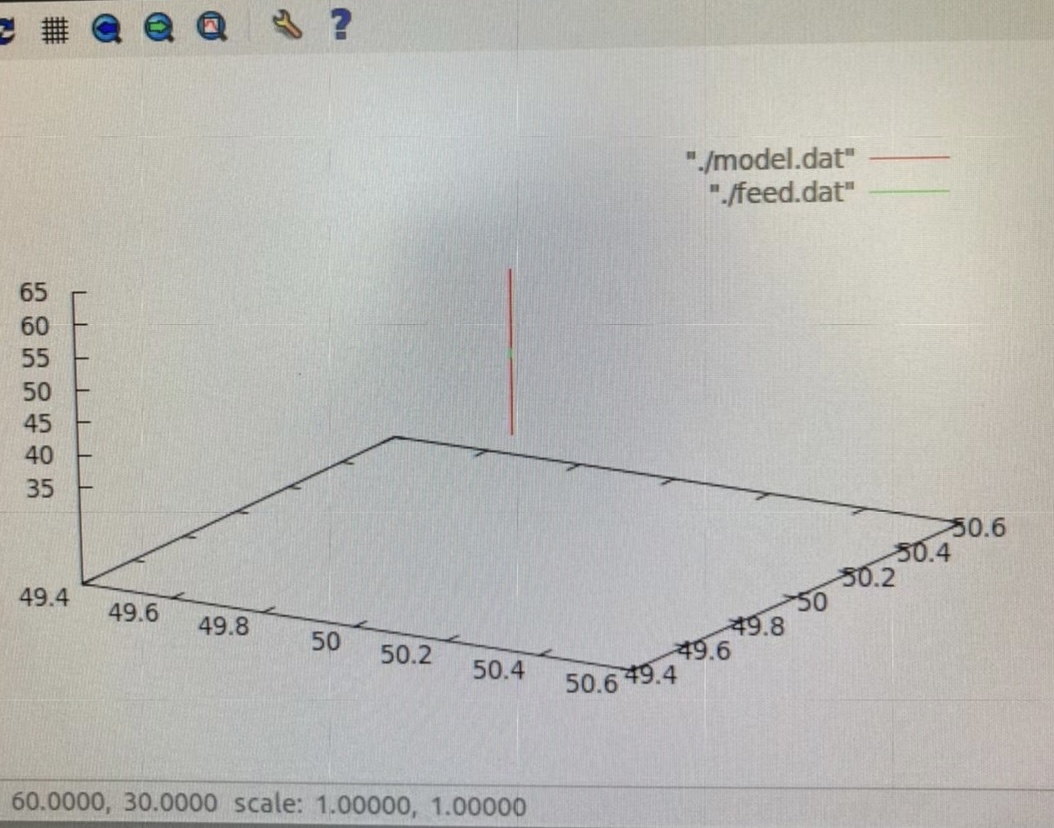
\includegraphics[scale=0.25]{fg1.jpg}
  \caption{モデリング}\label{fig:図1}
\end{figure}

\subsection{シミュレーション結果}

\subsubsection{電流}
グラフの横軸は時間、縦軸は電流の振幅を表す。下の図2より、電流は収束することが確認できた。\\
\begin{figure}[H]
  \centering
  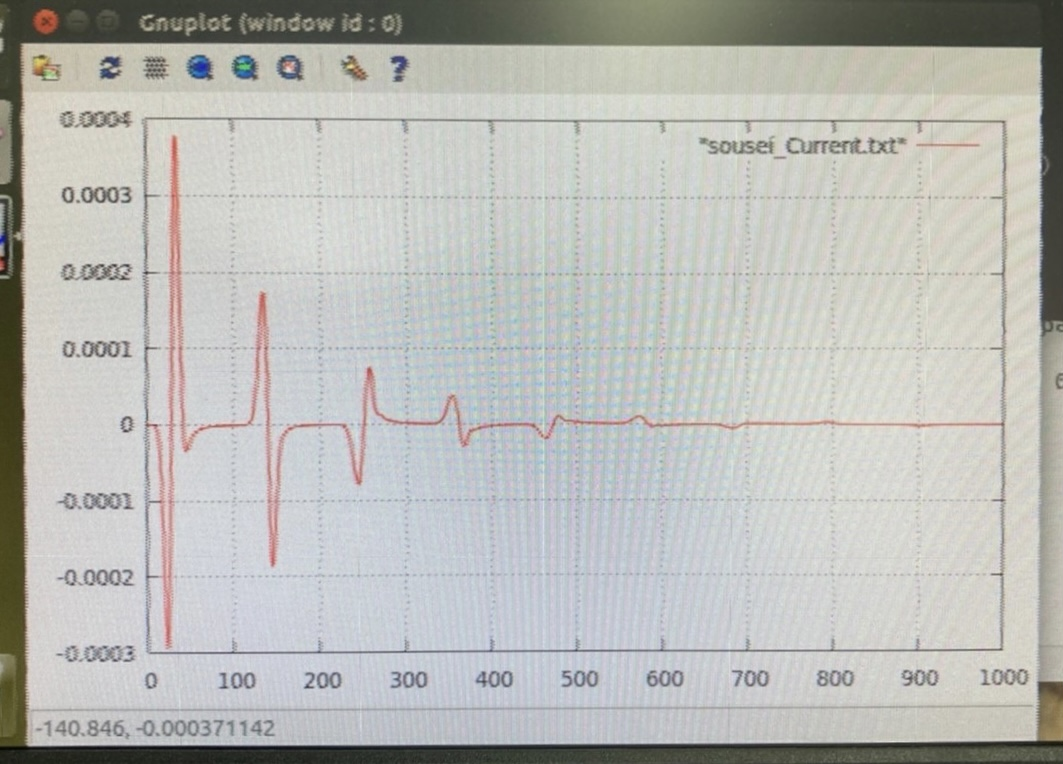
\includegraphics[scale=0.25]{fg5.jpg}
  \caption{電流}\label{fig:図2}
\end{figure}

\subsubsection{インピーダンス}
グラフの縦軸はインピーダンスの値、横軸は周波数を表す。また、赤線はインピーダンスの実部、緑線はインピーダンスの虚部を表す。インピーダンスの虚部が0になる周波数を共振周波数といい、基本的に動作させたい周波数でインピーダンスの実部が50Ω、虚部が0Ωになることを目指す。下の図3,4より、インピーダンスの実部が50Ωになるのは380-440MHzで、インピーダンスの虚部が0になるのは約460MHzであった。\\
\begin{figure}[H]
  \centering
  \begin{minipage}[b]{0.45\linewidth}
  \begin{center}
    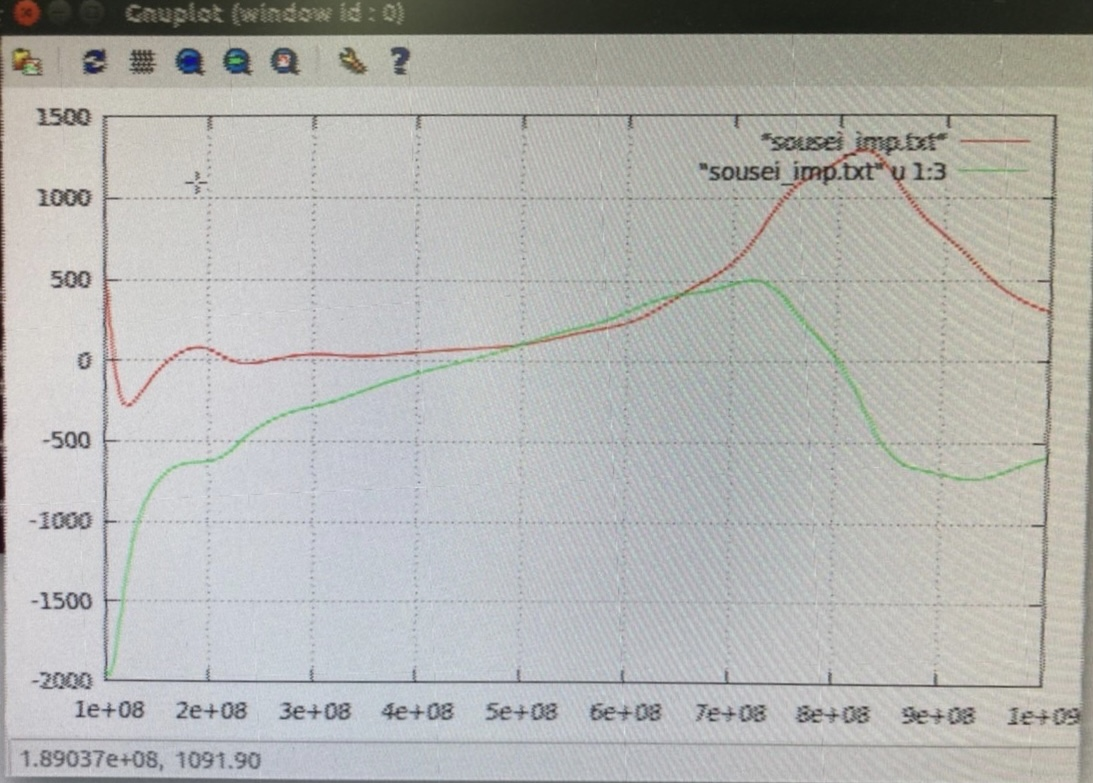
\includegraphics[keepaspectratio,scale=0.17]{fg6.jpg}
    \end{center}
    \caption{インピーダンス}
  \end{minipage}
  \begin{minipage}[b]{0.45\linewidth}
  \begin{center}
    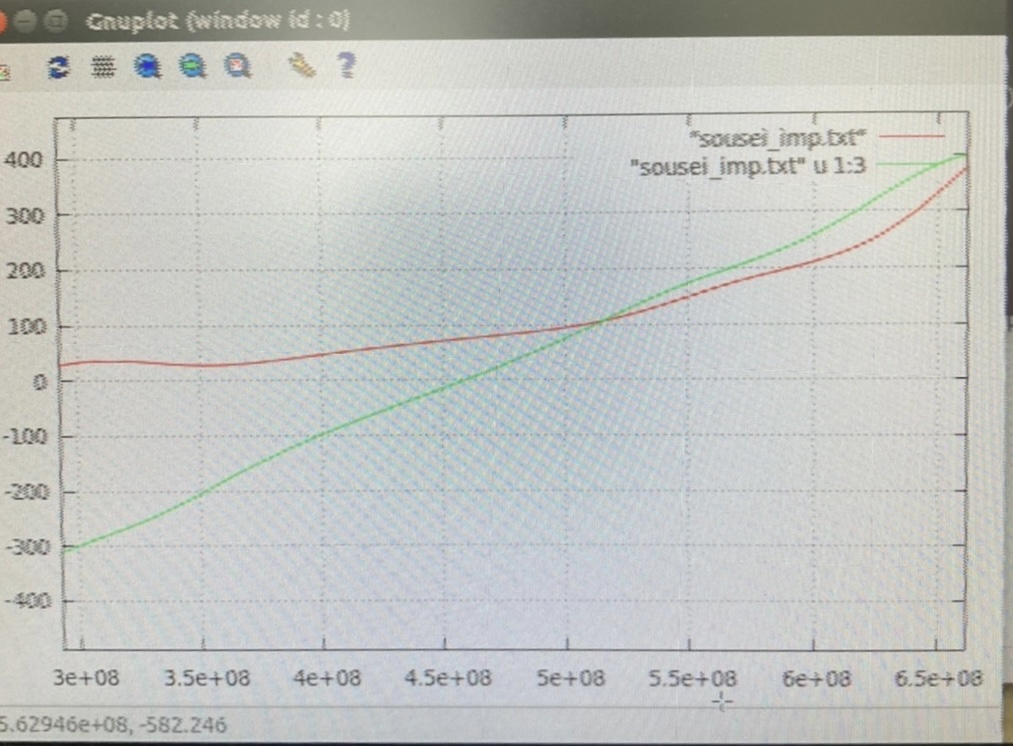
\includegraphics[keepaspectratio,scale=0.18]{fg7.jpg}
    \end{center}
    \caption{インピーダンス - 拡大}
  \end{minipage}
\end{figure}

\subsubsection{VSWR}
VSWRはインピーダンスの整合具合を表す指標の一つで、上記で確認したインピーダンスの関係を評価しやすい値に変換したものである。
インピーダンスの実部が50Ω、虚部が0ΩのときVSWRが1となり、これが最も良い値である。制作するアンテナはVSWRが目標の周波数で2以下になるよう設計する。
下の図5より、VSWRが最も1に近い値となったのは440MHzのときで、約1.5となった。しかし、目標である485MHzでは約3.0となり、アンテナの再設計が必要であることが分かった。\\
\begin{figure}[H]
  \centering
  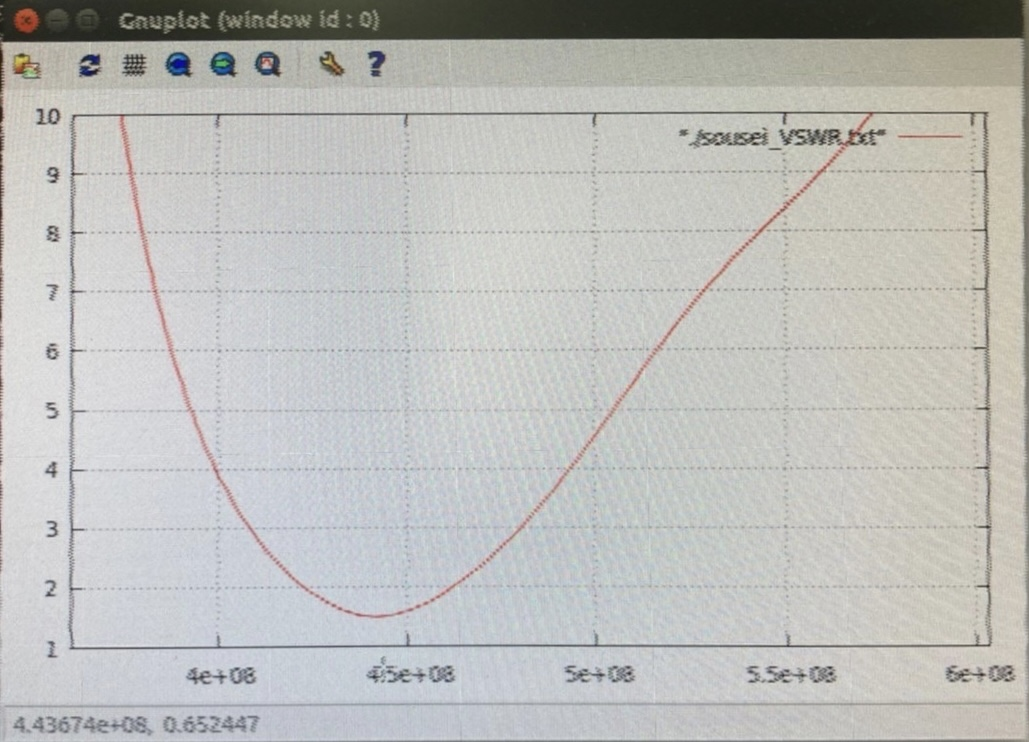
\includegraphics[scale=0.2]{fg8.jpg}
  \caption{VSWR}\label{fig:図5}
\end{figure}

\subsection{アンテナの改良}
\subsubsection{シミュレーション結果を受けて}
485MHzで設計したアンテナにおいて、VSWRが最も1に近くなったのは440MHzのときであった。このことから、半波長ダイポールアンテナは、計算に用いる周波数より低い周波数帯を拾いやすくなるのではないかと考えた。
このシミュレーションを考慮して、500MHzのダイポールアンテナを作れば、目標である485MHz付近で上手く動作すると予想した。
実際に設計とシミュレーションを行い、500MHzの半波長ダイポールアンテナのVSWRを求める。\\\\

\subsubsection{改良したアンテナのVSWR}
500MHzで設計し直した片側14.5cmのアンテナをシミュレーションしたものが下の図6,7である。VSMRは470MHzで最も1に近い値をとった。
目標であった485MHzにおいては、改良前のアンテナが約3.0であったのに対して、改良後は約1.5となり、目的の波長でVSWRが1に近付いた。\\
% よって、改良後のアンテナは目標の周波数においてより良く動作するアンテナだと言える。\\
\begin{figure}[H]
  \centering
  \begin{minipage}[b]{0.45\linewidth}
  \begin{center}
    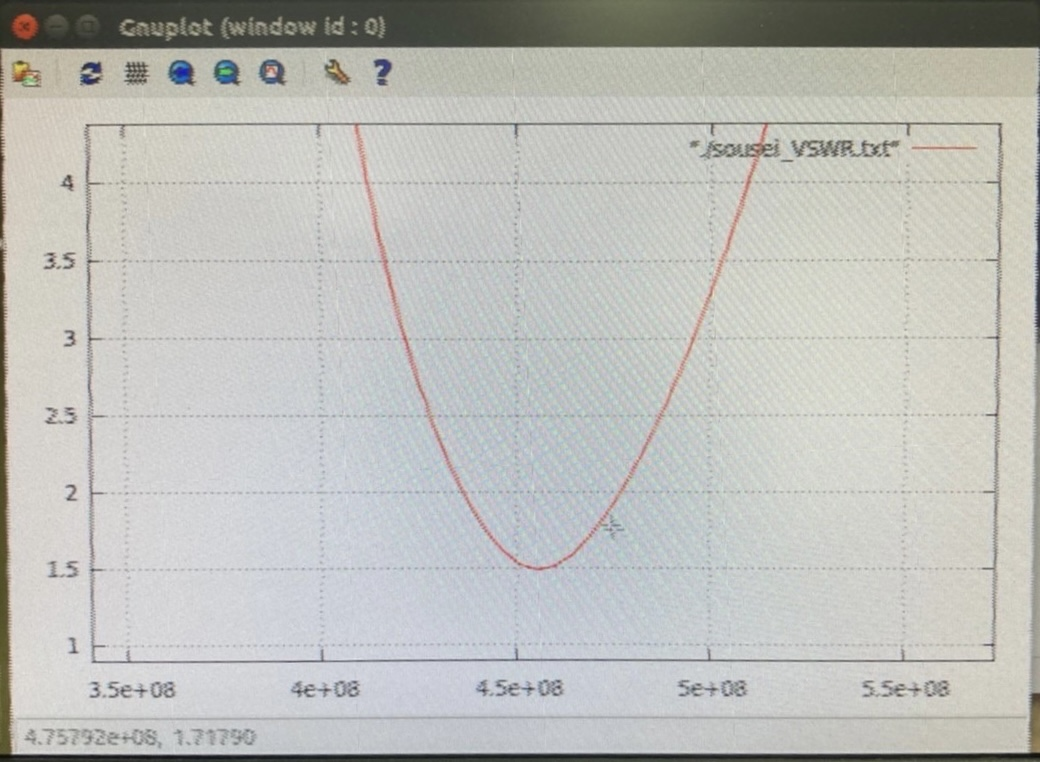
\includegraphics[keepaspectratio,scale=0.17]{fg9.jpg}
    \end{center}
    \caption{VSWR}
  \end{minipage}
  \begin{minipage}[b]{0.45\linewidth}
  \begin{center}
    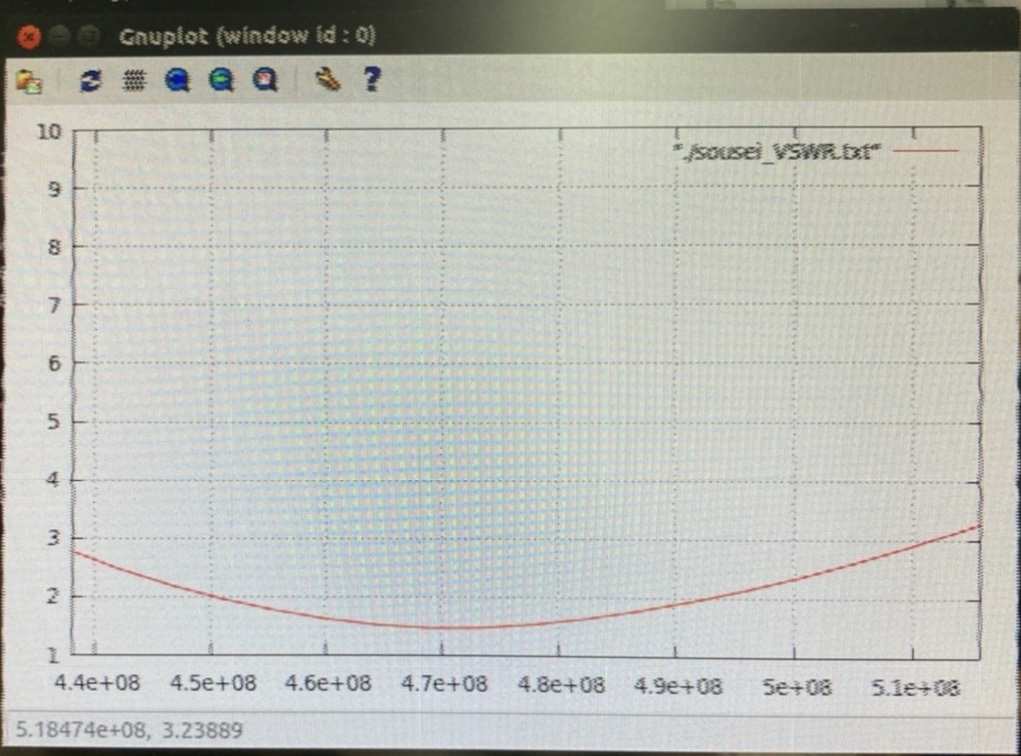
\includegraphics[keepaspectratio,scale=0.17]{fg10.jpg}
    \end{center}
    \caption{VSWR - 拡大}
  \end{minipage}
\end{figure}

\subsection{実験}
\subsubsection{アンテナの制作}
1.4章で設計を改良したアンテナを実際に制作した。エレメントには太さ2.0mmの銅線を使用し、それを同軸コネクタにボトルとナットを用い固定して給電部とした。
このとき、同軸コネクタ(給電部)を含むアンテナの全長がモデリングした長さと等しくなるようにしなければならない。
モデリングしたアンテナは両側のエレメントがそれぞれ14.5cm、給電部が1セル分の6mmで、全長が29.6cmである。一方で、実際の給電部は約1.5cmあったため、エレメントの長さをそれぞれ14cmに調整することで、アンテナの全長を約29.5cmに合わせた。\\

\subsubsection{地上デジタル放送の受信}
制作したアンテナを用いて、地上デジタル放送の受信と信号強度の測定を行った。信号強度とは受信されたワイヤレス信号の電波強度レベルを表す。
実験は別々の日に合わせて2回行った。下の表1が1回目、表2が2回目の実験結果である。1回目の実験では8つあるチャンネル中3つがテレビに映り、信号強度はKBS、BBC、YTVの順で高かった。
また、目標としてアンテナの設計を行ったABCは映すことができなかった。比べて、2回目の実験では8チャンネル全てのテレビ局を映すことができた。信号強度は上から4つがKBS、YTB、MBS、ABCであった。\\\\
1日目と2日目で信号強度の順番が入れかわったこと、2日目は目標としていたABCが比較的強い信号強度で受信できたことが確認できた。
また、8チャンネル中、YTBの信号強度は1日目は3番目に、2日目は2番目に高かった。設計したアンテナのVAWRが最も1に近かったのは470MHz付近であり、これはYTBの周波数帯も含まれる。\\

  \begin{table}[H]
    \centering
    \caption{測定結果-1回目}\label{fig:表1}
    \begin{tabular}{|c|c|c|}
    \hline
    放送局名       & 周波数範囲{[}MHz{]} & 信号強度{[}dB{]} \\ \hline
    NHK 大津総合   & 548-554        & ×            \\ \hline
    KBS 京都放送   & 530-536        & 6            \\ \hline
    BBC  びわ湖放送 & 512-518        & 3            \\ \hline
    KTV 関西テレビ  & 494-500        & ×            \\ \hline
    MBS 毎日放送   & 488-494        & ×            \\ \hline
    ABC 朝日放送   & 482-488        & ×            \\ \hline
    YTV 読売テレビ  & 476-482        & 0            \\ \hline
    NHK 大阪教育   & 470-476        & ×            \\ \hline
    \end{tabular}
    \end{table}

  \begin{table}[H]
    \centering
    \caption{測定結果-2回目}\label{fig:表2}
    \begin{tabular}{|c|c|c|}
    \hline
    放送局名       & 周波数範囲{[}MHz{]} & 信号強度{[}dB{]} \\ \hline
    NHK 大津総合   & 548-554        & 0            \\ \hline
    KBS 京都放送   & 530-536        & 14            \\\hline
    BBC  びわ湖放送 & 512-518        & 5            \\\hline
    KTV 関西テレビ  & 494-500        & 0            \\\hline
    MBS 毎日放送   & 488-494        & 7            \\\hline
    ABC 朝日放送   & 482-488        & 6            \\\hline
    YTV 読売テレビ  & 476-482        & 8            \\\hline
    NHK 大阪教育   & 470-476        & 4            \\ \hline
    \end{tabular}
    \end{table}

\subsection{考察}
2回の実験は同じアンテナと場所で測定を行なったが、テレビやケーブルなどの機材が異なったことが影響し、受信できたチャンネル数(帯域幅)や信号強度に大きな違いがあった。
しかし、KBS、BBCが強く受信できたこと、YTBが受信できたことは共通している。このことについて、KBS、BBCが受信できた要因と、YTBが受信できた要因は別であると予想した。
まず、KBS、BBCの周波数帯ではアンテナのVSWRが4を超えていることから、本来アンテナはうまく動作しないはずである。しかし、KBS、BBCは基地局からの送信電力が強いため、信号強度も強くなったのではないかと考えた。
一方で、YTBは送信電力は強くないが、周波数範囲476-482HMzと、今回設計したアンテナが最も良く動作する周波数であったため、受信することが出来たのではないかと考えた。\\\\\\\\

\section{5th week 改良アンテナのシミュレーション}
\subsection{概要}
1章で製作した半波長ダイポールアンテナより良いアンテナを設計して製作を行う。
製作するアンテナを定めるために、3種類のアンテナを設計し、シミュレーションすることにした。アンテナの種類は、より高い利得を有するアンテナとして反射板付きダイポールアンテナ、八木・宇田アンテナを、より広帯域を受信するアンテナとして折返しアンテナを選択した。
今回、受信を目的とするのはBBCびわ湖放送(512-518MHz)である。1章で半波長ダイポールアンテナは設計した周波数より低い周波数で良く機能したため、比較的高い周波数帯で、下の周波数帯に多くのチャンネルがあるBBCが適切であると考えた。\\

\subsection{反射板付きダイポールアンテナ}
\subsubsection{概要}
反射板付きダイポールアンテナは、半波長ダイポールアンテナを放射器とし、金属板を反射器とするアンテナである。
後方に放射した電波を前方に反射することによって、前方に高い利得の電波を放射する。\\\\
\begin{figure}[H]
  \centering
  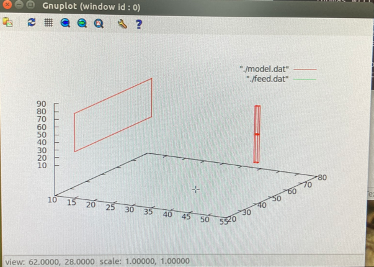
\includegraphics[scale=0.6]{i1.png}
  \caption{モデリング}\label{fig:図10}
\end{figure}

\subsubsection{VSWR}
下の図9より、約430MHzから470MHzで高い利得が得られた。最も1に近い値となったのは450MHzで約1.1であった。\\
\begin{figure}[H]
  \centering
  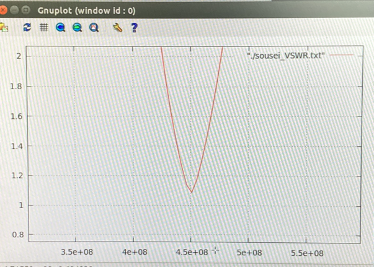
\includegraphics[scale=0.6]{i2.png}
  \caption{VSWR}\label{fig:図11}
\end{figure}

\subsubsection{指向性}
アンテナはz軸に沿って伸びているので、アンテナに垂直な平面であるxy平面を見ると、反射板からみて放射器の方向に、斜め2方向に分かれて指向性が高くなっている。\\
\begin{figure}[H]
  \centering
  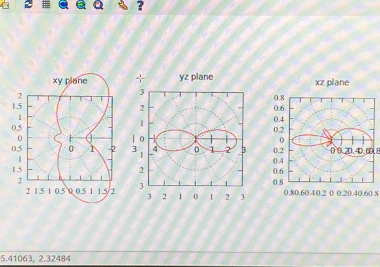
\includegraphics[scale=0.6]{i3.png}
  \caption{指向性}\label{fig:図12}
\end{figure}


\subsection{八木・宇田アンテナ}
\subsubsection{概要}
八木・宇田アンテナは後方に反射器、中央に放射器、前方に放射器を並べた構造のアンテナであり、強い利得を有する。反射器の太さや導波器の個数、エレメント間の間隔などが様々なものがあり、それにより特性が変化する。
今回のシミュレーションでは反射器を用いず、下の図11のように放射器と導波器の2つのエレメントを用いて設計した。これにより、導波器にどの程度効果があるか確認したい。\\
\begin{figure}[H]
  \centering
  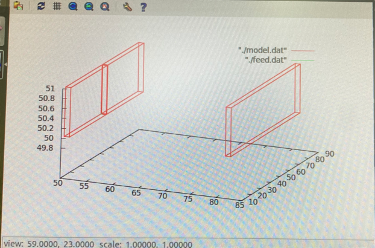
\includegraphics[scale=0.6]{yagi1.png}
  \caption{モデリング}\label{fig:図13}
\end{figure}

\subsubsection{VSWR}
下の図12より、約430MHzから480MHzで非常に高い利得が得られた。最も1に近い値となったのは450MHzで約1.0であった。\\
\begin{figure}[H]
  \centering
  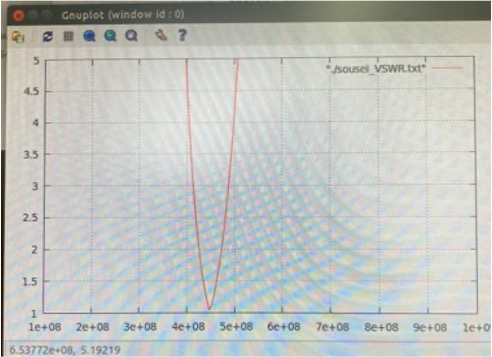
\includegraphics[scale=0.45]{yagi2.jpg}
  \caption{VSWR}\label{fig:図14}
\end{figure}

\subsubsection{指向性}
アンテナはy軸に沿って伸びているので、アンテナに垂直な平面であるxz平面を見ると、z軸方向に指向性が見られた。
\begin{figure}[H]
  \centering
  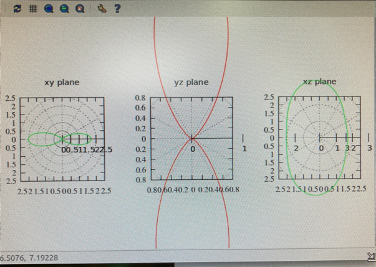
\includegraphics[scale=0.6]{yagi3.png}
  \caption{指向性}\label{fig:図15}
\end{figure}

\subsection{折返しアンテナ}
\subsubsection{概要}
折り返しアンテナは、アンテナのパラメーターを変えることによりインピーダンスの調節ができるアンテナです。このインピーダンス
調整の指標をstep up ratioという。\\
\begin{figure}[H]
  \centering
  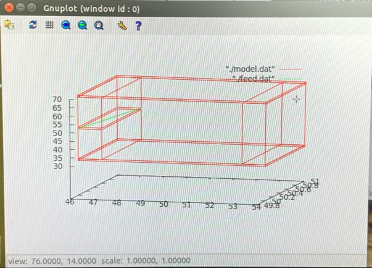
\includegraphics[scale=0.6]{o1.png}
  \caption{モデリング}\label{fig:図16}
\end{figure}

\subsubsection{VSWR}
他の2つのアンテナほど高い利得を得られる帯域が存在しなかった。\\
\begin{figure}[H]
  \centering
  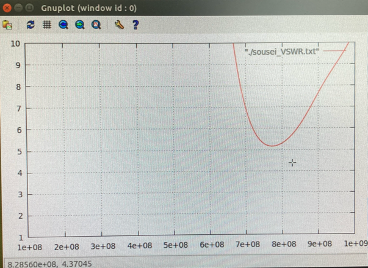
\includegraphics[scale=0.6]{o2.png}
  \caption{VSWR}\label{fig:図17}
\end{figure}

\subsubsection{指向性}
下の図16のxy平面のグラフから、給電点側に指向性があるのが分かる。\\
\begin{figure}[H]
  \centering
  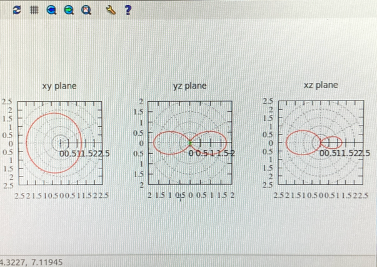
\includegraphics[scale=0.6]{o3.png}
  \caption{指向性}\label{fig:図18}
\end{figure}

\subsection{アンテナ製作の方針}
上記の3つのアンテナのシミュレーション結果から、高い利得が得られる周波数範囲が最も広いことと、高い指向性が得られたことから、八木・宇田アンテナを製作することに決定した。
反射板付きダイポールアンテナも概ね良いシミュレーション結果を得られたが、金属板の準備などの観点も含めて却下した。\\\\\\\\

\section{6-7 week 八木・宇田アンテナ}
\subsection{概要}
第2章のシミュレーションの結果を踏まえ、八木・宇田アンテナの製作を行う。
今回の実験では、八木・宇田アンテナに本来存在する反射器を用いず、放射器と導波器だけでどのような結果になるか観測する。ただし、比較対象として反射器も用いた八木・宇田アンテナのシミュレーションも行い、どの程度指向性に違いが出るかを確認する。\\

\subsection{アンテナの設計}
BBCびわ湖放送の周波数範囲が512-518MHzであるので、中心周波数の514MHzで波長の計算を行った。
\begin{eqnarray*}
  \lambda = \frac{3.0 \times 10^8 [m/s]}{5.14 \times 10^8 [m/s]} = 0.584[m] = 58.4[cm]\\
\end{eqnarray*}

放射器には半波長ダイポールアンテナを使用する。
2本のエレメントの長さはそれぞれ1/4λなので、14.6cmでとなる。それに4mmの給電点を合わせた全体の長さが29.6cmのアンテナを設計した。
また、放射器が0.5λより、配布された資料の「Three-element Yagi-Uda dipole antenna」を参考に、反射器の長さを0.52λ、導波器の長さを0.48λと設計した。
下の図17,18はそれぞれ反射器なし、反射器ありの八木・宇田アンテナの設計図である。\\

\begin{figure}[H]
  \centering
  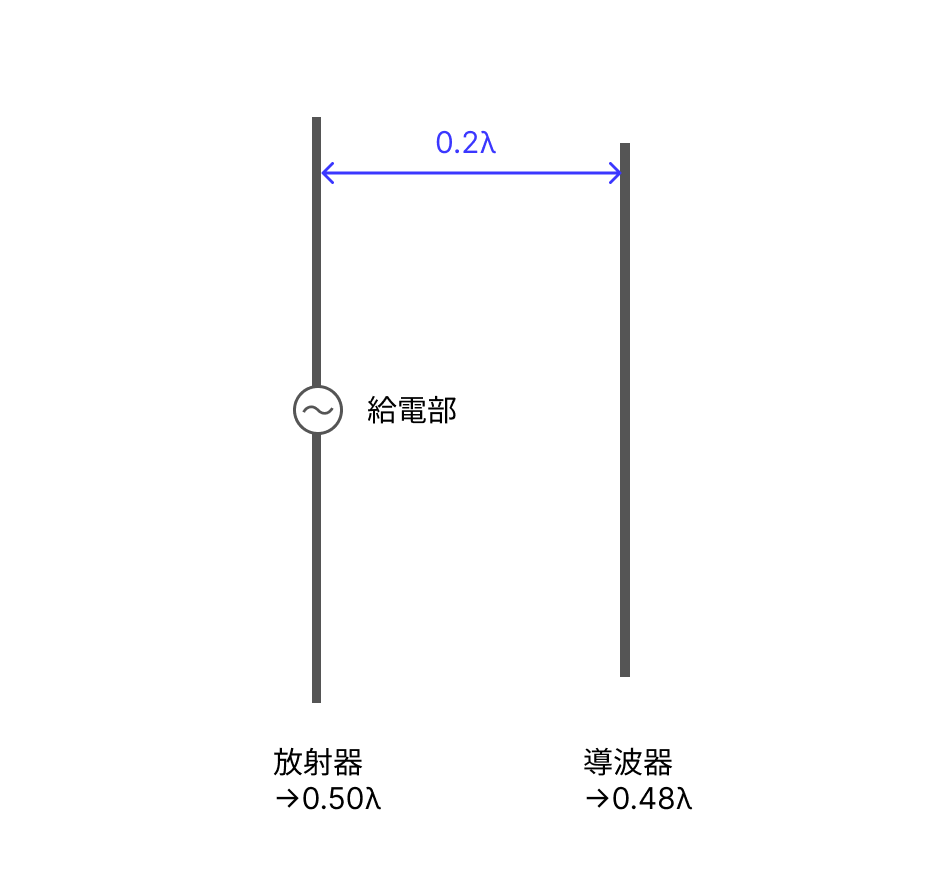
\includegraphics[scale=0.28]{yagiuda.png}
  \caption{反射器なし}\label{fig:図19}
\end{figure}

\begin{figure}[H]
  \centering
  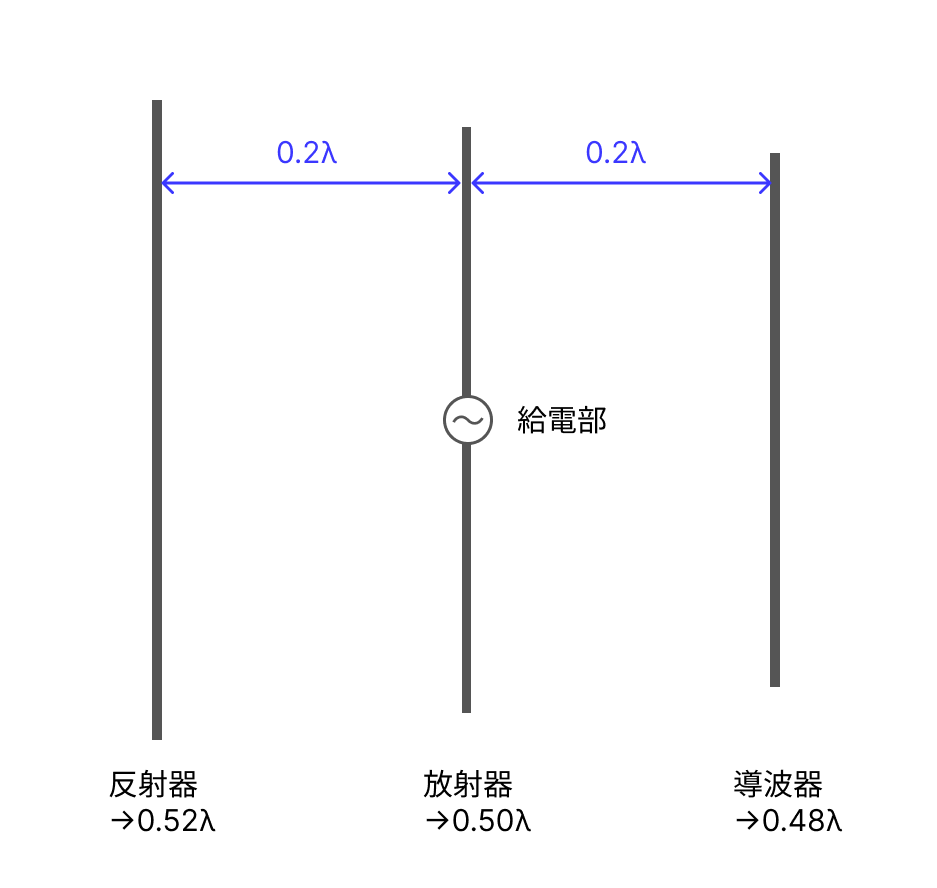
\includegraphics[scale=0.28]{yagiuda1.png}
  \caption{反射器あり}\label{fig:図20}
\end{figure}

また、下の図19,20はそれぞれ反射器なし、反射器ありの八木・宇田アンテナのモデリング結果である。\\\\\\

\begin{figure}[H]
  \centering
  \begin{minipage}[b]{0.45\linewidth}
  \begin{center}
    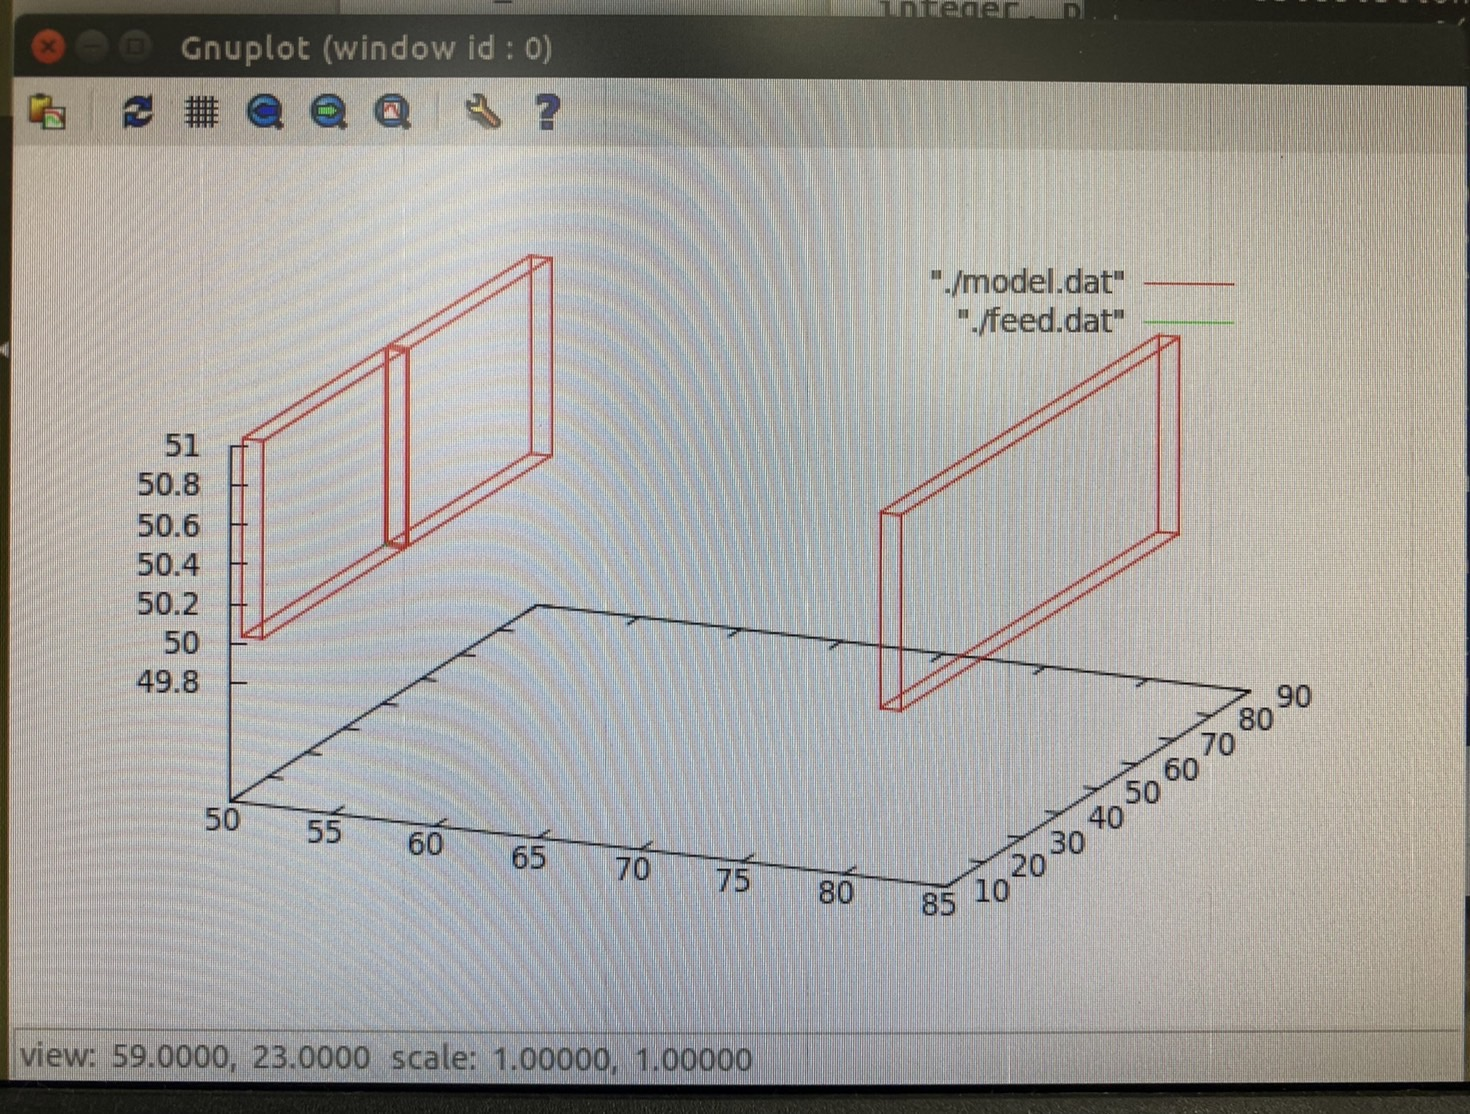
\includegraphics[keepaspectratio,scale=0.13]{s1.jpg}
    \end{center}
    \caption{反射器なし}
  \end{minipage}
  \begin{minipage}[b]{0.45\linewidth}
  \begin{center}
    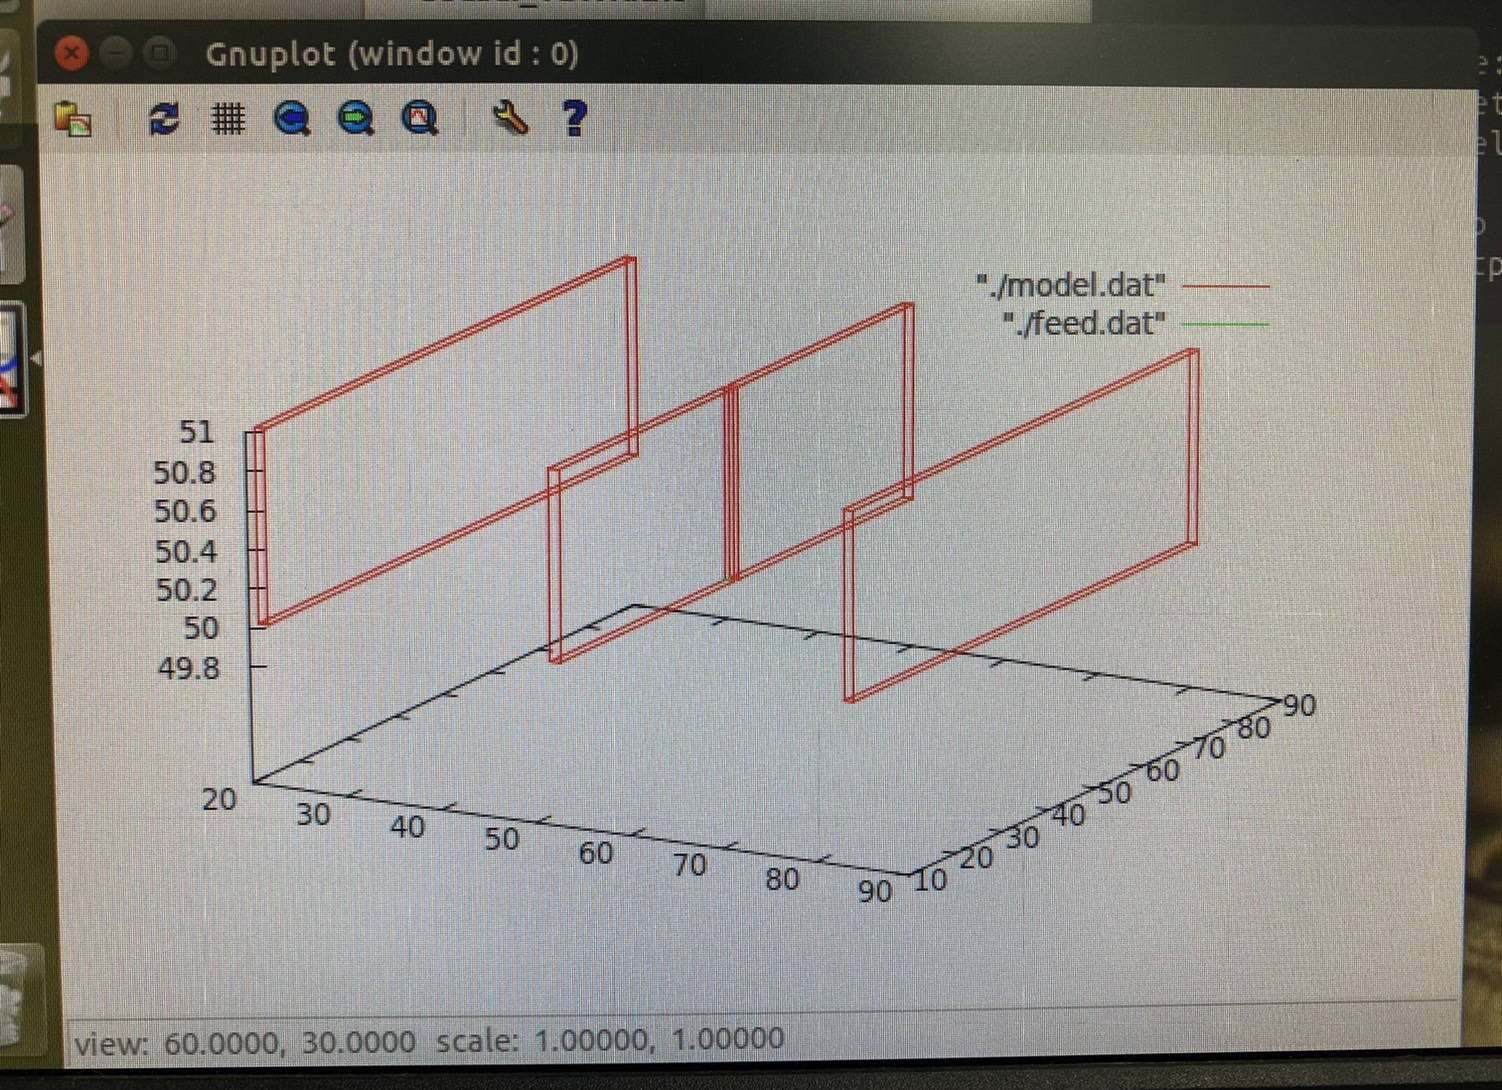
\includegraphics[keepaspectratio,scale=0.13]{s2.jpg}
    \end{center}
    \caption{反射器あり}
  \end{minipage}
\end{figure}

\subsection{シミュレーション結果}
\subsubsection{VSWR}
図21,22より、反射器なしのアンテナは430MHzから480MHzで非常に高い利得、反射器ありのアンテナは430MHzから460MHzで高い利得を得られることが分かった。\\

\begin{figure}[H]
  \centering
  \begin{minipage}[b]{0.45\linewidth}
  \begin{center}
    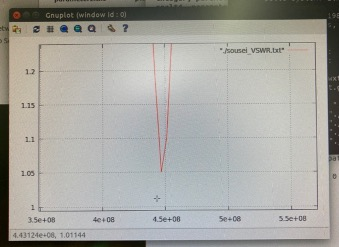
\includegraphics[keepaspectratio,scale=0.5]{fg11.jpg}
    \end{center}
    \caption{反射器なし}
  \end{minipage}
  \begin{minipage}[b]{0.45\linewidth}
  \begin{center}
    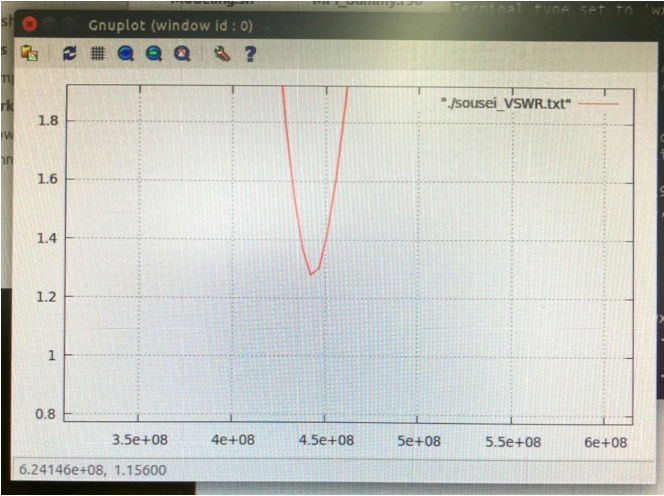
\includegraphics[keepaspectratio,scale=0.5]{fg12.png}
    \end{center}
    \caption{反射器あり}
  \end{minipage}
\end{figure}

\subsubsection{指向性}
アンテナに垂直な平面であるxz平面を見ると、どちらもz軸方向に指向性があった。特に、反射器ありのアンテナの方が鋭い指向性があった。\\
\begin{figure}[H]
  \centering
  \begin{minipage}[b]{0.45\linewidth}
  \begin{center}
    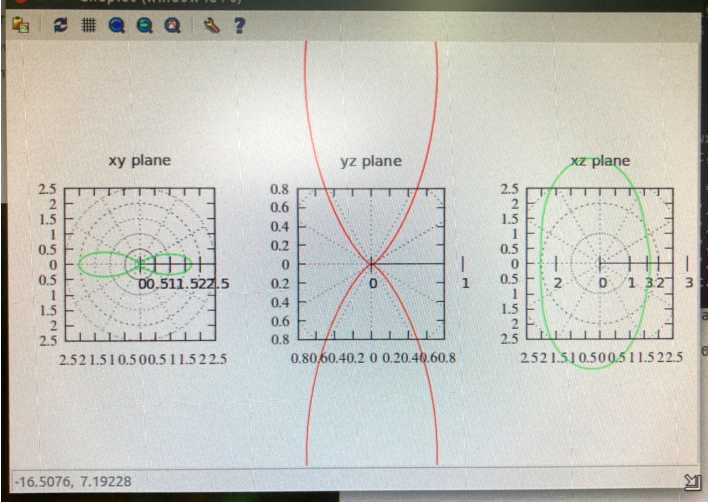
\includegraphics[keepaspectratio,scale=0.5]{fg13.png}
    \end{center}
    \caption{反射器なし}
  \end{minipage}
  \begin{minipage}[b]{0.45\linewidth}
  \begin{center}
    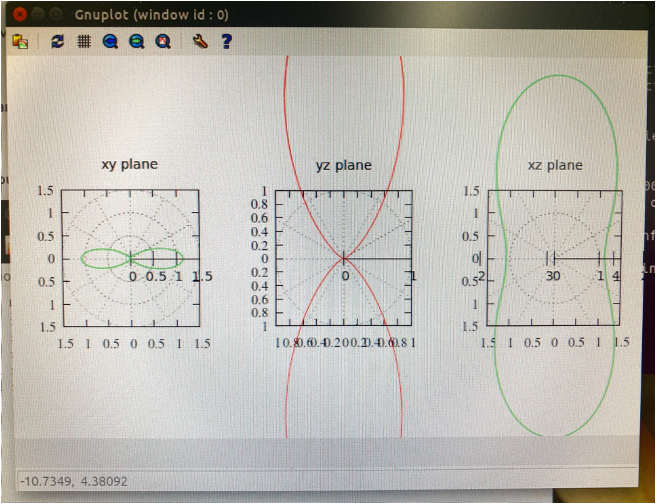
\includegraphics[keepaspectratio,scale=0.5]{fg14.png}
    \end{center}
    \caption{反射器あり}
  \end{minipage}
\end{figure}

\subsection{地上デジタル放送の受信}
実際に反射板なしの八木・宇田アンテナで地上デジタル放送の受信と信号強度の測定を行った。アンテナを地上に対して水平に寝かせ、建物内から外に向かって電波を受信した。
また、放射器と導波器の位置関係が電波受信に与える影響を調べるため、導波器を外側にした場合(外向き)と、建物側にした場合(内向き)で2回測定を行った。
表3,4より、KBSについては反波長ダイポールアンテナよりかなり高い信号強度で受信することが出来たことが分かる。しかし、目標としたBBCや、VSWRで高い利得を確認できた周波数帯に関しては、ほとんど変化がなかった。\\


\begin{table}[H]
  \centering
  \caption{測定結果-外向き}\label{fig:表3}
  \begin{tabular}{|c|c|c|}
  \hline
  放送局名       & 周波数範囲{[}MHz{]} & 信号強度{[}dB{]} \\ \hline
  NHK 大津総合   & 548-554        & ×            \\ \hline
  KBS 京都放送   & 530-536        & 22            \\ \hline
  BBC  びわ湖放送 & 512-518        & 2            \\ \hline
  KTV 関西テレビ  & 494-500        & 0            \\ \hline
  MBS 毎日放送   & 488-494        & ×            \\ \hline
  ABC 朝日放送   & 482-488        & ×            \\ \hline
  YTV 読売テレビ  & 476-482        & 0            \\ \hline
  NHK 大阪教育   & 470-476        & ×            \\ \hline
  \end{tabular}
  \end{table}

  \begin{table}[H]
    \centering
    \caption{測定結果-内向き}\label{fig:表4}
    \begin{tabular}{|c|c|c|}
    \hline
    放送局名       & 周波数範囲{[}MHz{]} & 信号強度{[}dB{]} \\ \hline
    NHK 大津総合   & 548-554        & ×            \\ \hline
    KBS 京都放送   & 530-536        & 27            \\ \hline
    BBC  びわ湖放送 & 512-518        & 5            \\ \hline
    KTV 関西テレビ  & 494-500        & ×            \\ \hline
    MBS 毎日放送   & 488-494        & 4            \\ \hline
    ABC 朝日放送   & 482-488        & ×            \\ \hline
    YTV 読売テレビ  & 476-482        & 1            \\ \hline
    NHK 大阪教育   & 470-476        & ×            \\ \hline
    \end{tabular}
    \end{table}


\subsection{考察}
八木・宇多アンテナの測定結果が、シミュレーションから期待されたものと異なる結果になった原因について考察した。
電波には、送信局からの電波の送信方式(縦波、横波)の違いにより、水平偏波と垂直偏波がある。今回の実験では、八木・宇多アンテナを地面と水平になるよう寝かせて実験を行ったが、水平偏波時はアンテナの導波器(素子)が水平に、
垂直偏波時はアンテナの導波器(素子)が垂直になるように設置しなければならなかった。今回受信した放送局は垂直偏波であったのに対し、アンテナを水平にしてしまったことで、指向性の高さを活かせなかったのではないかと考えた。\\

\section{付録}
\subsection{メモ-1回目}
はじめに先週の説明を受けて分からなかったことを質問し、parameter.txtやmodeling.txtについて、パラメータの設定や関数の役割を理解することができた。その後、2週目の内容である1GHzの半波長ダイポールアンテナの計算を開始した。

まず、周波数が1GHzのときの波長を求め、そこからセルに換算して、ダイポールアンテナをモデリングした。モデリングしたアンテナを用いて計算を行い、souseiのデータファイルが更新されたので、それぞれの値について描画を行った。

グラフを確認したところ、アンテナは全く同じものをモデリングしたはずが、インピーダンスやVSWR、指向性パターンがテキストとかなり異なる結果になっていた。parameter.txtを再度確認したところ、1セルの設定が6mmではなく2mmになっていた。シュミレーションした際の計算時間が長かったのも、そのためだということが分かった。

セルの長さが1/3になっていたということは、半波長のアンテナをシュミレーションしたつもりが、6分の1波長のアンテナをシュミレーションしてしまった事になる。また、他の設定にも影響を与えてしまっていた。しかし、この計算で得られた結果も比較対象のデータとして残すことにした。

その後、parameter.txtの中身をテキストと同じにして計算を行い、グラフで結果を確認したところ、今度はテキストと同じグラフを示した。

最後に、parameter.txtの測定領域を変え、折り返しアンテナをモデリングした。始点と終点を決め、setboxを用いることで厚みのあるアンテナがモデリングできると分かった。

シュミレーションすると、インピーダンスの虚部が0になるときがなかったり、VSWRの値が最小でも8であったりと、このままでは良いアンテナとは言えないことが分かった。次回の作業では、parameter.txtを設定することで、この折り返しアンテナを良いアンテナに近づけたい。\\\\


\subsection{メモ-2回目}
本日の実験では、特定の放送チャンネルが映るようなダイポールアンテナを設計した。
初めに、映したい放送チャンネルをABC朝日放送(以下ABC)と定めた。ABCにした理由は、ABCの使用する周波数範囲の付近は、他の放送チャンネルも多いので、受信周波数がABCの周波数に合わなかった場合も、他のチャンネルが映る可能性が高いと考えたからである。

次に、ABCの使用する周波数範囲である482~488MHzで動作するようなダイポールアンテナを設計し、シミュレーションをおこなった。485MHzを受信する片側15.5cmのアンテナで計算したところ、VSWRが最も1に近くなったのは440MHzのときであった。このことから、設計したアンテナは想定より低い周波数を拾いやすいことが分かった。

一度目におこなったシミュレーションを考慮して、500MHzのダイポールアンテナを作れば、目標である485MHzで上手く動作すると予想した。500MHzで設計し直した片側14.5cmのアンテナをシミュレーションすると、470MHzでVSMRが最も1に近づき、目標であった485MHzでも2以下の値となった。\\\\

\subsection{メモ-3回目}
今回の実験では、はじめに前回製作した半波長ダイポールアンテナを使って、地上デジタル放送の受信を再び行なった。同じアンテナと場所で測定を行なったが、テレビなど前回とは別の機材を使ったことが影響して、受信できたチャンネル数(帯域幅)や受信電力に大きな違いがあった。

前回の測定で受信できたのは8チャンネル中3チャンネルで、BBCびわ湖が3dB、YTB読売テレビが1dB、KBS京都が6dBであった。アンテナを設計する際に採用した波長の周波数帯域にあるABC朝日放送は受信することができなかった。
比べて、今回の実験では8チャンネル全てのテレビ局の電波を受信することができた。具体的には、NHK大津総合が0dB、NHK大阪教育が4dB、BBCびわ湖が5dB、MBS毎日放送が7dB、ABC朝日放送が6dB、KTB関西テレビが0dB、YTB読売テレビが8dB、KBS京都が14dBで受信できた。全ての放送局が前回の測定より映ること、目標としたABC朝日放送が比較的強い電波強度で受信できることが確認できた。

今回の結果を採用するならば、作成したアンテナは地上放送を受信するのに十分な帯域を受信できるとし、アンテナ改良の目標として、より受信電力を上げることや、性能を上げることを目標にすべきだと考えた。

最後に、次回から製作するアンテナを定めるために、班の3人でそれぞれ1つずつアンテナを設計し、3種類のアンテナをシミュレーションすることにした。アンテナの種類は、より高い利得を有するアンテナとして八木・宇田アンテナと反射板付きダイポールアンテナを、より広帯域を受信するアンテナとして折返しアンテナを選択した。

私はその中で八木・宇田アンテナの設計を担当することになり、反射器や導波器の長さを決めるために、まず参考資料を探した。すると、反射器や導波器の長さや、放射器との間隔が異なるものが数個見つかった。これは八木・宇田アンテナが良く機能する値がいくつか見つかっているためだと分かった。また、資料によると反射器の太さや導波器の個数によってアンテナの特性が変化するので、色々な構造が検討できるとのことだった。そこで、基準を作るためにも放射器と導波器だけのシンプルな構造でアンテナを設計してみることにした。放射器は前回設計したものと同じ半波長ダイポールアンテナとし、そこに導波器を加えることでどのような変化が見られるかを調べたい。放射器と導波器の間隔を0.2波長とし、導波器はいくつか異なる長さで試すことにした。

また他の比較対象として、同じ半波長ダイポールアンテナを使用し、放射器と導波器ではなく、放射器と反射板を用いる反射板付きダイポールアンテナとの違いにも注目したい。\\\\

\subsection{メモ-4回目}
はじめに、次回の授業時間を無駄なく使い、実験とレポートに必要なデータの収集を完了させるために、チームメンバーと計画を立て直した。当初は、3人がそれぞれ設計してきた八木・宇田アンテナ、折り返しアンテナ、反射板付きダイポールアンテナをコンピュータでシミュレーションして、その結果から作成するアンテナを決め、アンテナの作成と実験を行う予定だったが、これでは時間が足りないと考えた。そこで、反射板の大きさの調整に時間がかかるであろう反射板付きダイポールアンテナは、作成する可能性が低いことから、シミュレーションの優先度を下げ、八木・宇田アンテナと折り返しアンテナのシミュレーションが終わり次第、アンテナの作成に移ることにした。

また、八木・宇田アンテナの場合は以前作成した半波長ダイポールアンテナを放射器に再利用することで、アンテナの作成時間の短縮と、前回との比較実験になるのではないかと考えた。しかし、作成した半波長ダイポールアンテナは実験を行う中で長さを短くする調整を行ったので、それに合わせてアンテナのモデリングをやり直す必要があり、新たなものを作成した方が確実だという意見もあった。

最後に、今週の講義を受けて、先週作成した八木・宇田アンテナの設計を見直した。\\
\end{document}